%---------------------------------------------
%    PACKAGES AND THEMES
%---------------------------------------------

\documentclass[aspectratio=169,xcolor=dvipsnames,10pt]{beamer}
\usetheme{Madrid}
\usecolortheme{default}

\usepackage{hyperref}
\usepackage{graphicx}
\usepackage{booktabs}
\usepackage{amsmath}
\usepackage{amssymb}
\usepackage{tikz}
\usepackage{array}
\usepackage{multirow}
\usetikzlibrary{shapes.geometric, arrows.meta, positioning, calc, fit, backgrounds}

%--------------------------------------
%    TITLE PAGE
%--------------------------------------

\title[Sentiment Analysis \& BI Extraction]{Automated Sentiment Analysis and Topic Modelling\\for E-Commerce Business Intelligence Extraction}

\author[Akshat Kumar Nayak]{
    \textbf{Akshat Kumar Nayak} \\
    \vspace{0.1cm} Roll No: 2022BCS-005 \\
    \vspace{0.5cm}
    \small{\textit{Under the supervision of}} \\
    \textbf{Dr. Santosh Singh Rathore}
}

\institute{
    Department of Computer Science \& Engineering \\
    \vspace{0.2cm}
    \textit{B.Tech Project Presentation}
}
\date{May 2026}

%----------------------------------------
%    PRESENTATION SLIDES
%----------------------------------------

\begin{document}

%------------------------------------------------------------
% Slide 1: Title
%------------------------------------------------------------
\begin{frame}
    \titlepage
\end{frame}

%------------------------------------------------------------
% Slide 2: Table of Contents
%------------------------------------------------------------
\begin{frame}{Outline}
    \tableofcontents
\end{frame}

%============================================================
\section{Introduction \& Motivation}
%============================================================

\begin{frame}{Introduction \& Motivation}
    \begin{columns}[T]
        \column{0.55\textwidth}
        \begin{block}{The E-Commerce Review Problem}
            \footnotesize
            \begin{itemize}
                \item Global e-commerce market surpassed \textbf{\$5.8 trillion} in 2023, growing at 10\%+ CAGR.
                \item \textbf{93\%} of consumers read reviews before purchase; 1-star improvement $\rightarrow$ \textbf{5--9\% revenue gain}.
                \item Amazon hosts \textbf{hundreds of millions} of reviews --- impossible to analyse manually.
            \end{itemize}
        \end{block}

        \vspace{0.4em}
        \begin{alertblock}{Why Existing Systems Fall Short}
            \footnotesize
            \begin{itemize}
                \item \textbf{Star ratings alone} discard rich textual signal.
                \item \textbf{Domain mismatch}: models trained on movie reviews misclassify informal product language.
                \item \textbf{Implicit negativity} (``I guess it works'') missed by naive lexicons.
                \item \textbf{No actionable BI}: accuracy metrics, not business recommendations.
            \end{itemize}
        \end{alertblock}

        \column{0.42\textwidth}
        \begin{exampleblock}{This Project Proposes}
            \footnotesize
            An integrated end-to-end pipeline that:
            \begin{enumerate}
                \item Fuses multiple sentiment models for improved accuracy
                \item Applies neural topic modelling (BERTopic)
                \item Extracts structured BI (priority matrices, scorecards, aspect sentiment)
                \item Serves results via interactive dashboard + LLM agent
            \end{enumerate}
        \end{exampleblock}
    \end{columns}
\end{frame}

%============================================================
\section{Dataset \& Preprocessing}
%============================================================

\begin{frame}{Dataset}
    \begin{columns}[T]
        \column{0.50\textwidth}
        \begin{block}{Amazon Product Reviews}
            \footnotesize
            \begin{itemize}
                \item \textbf{172,718 reviews} across \textbf{6 categories}
                \item Each record: review text, star rating (1--5), category, reviewer ID, timestamp
                \item Balanced sampling ($\sim$28,786 per category)
            \end{itemize}
        \end{block}

        \vspace{0.5em}
        \footnotesize
        \begin{tabular}{|l|c|c|}
            \hline
            \textbf{Category} & \textbf{Reviews} & \textbf{Avg Rating} \\
            \hline
            Electronics            & $\sim$28,786 & 3.9 \\
            Home \& Kitchen        & $\sim$28,786 & 4.1 \\
            Clothing               & $\sim$28,786 & 4.0 \\
            Sports \& Outdoors     & $\sim$28,786 & 4.2 \\
            Grocery \& Gourmet     & $\sim$28,786 & 4.3 \\
            Toys \& Games          & $\sim$28,786 & 4.1 \\
            \hline
            \textbf{Total}         & \textbf{172,718} & \textbf{4.1} \\
            \hline
        \end{tabular}

        \column{0.47\textwidth}
        \centering
        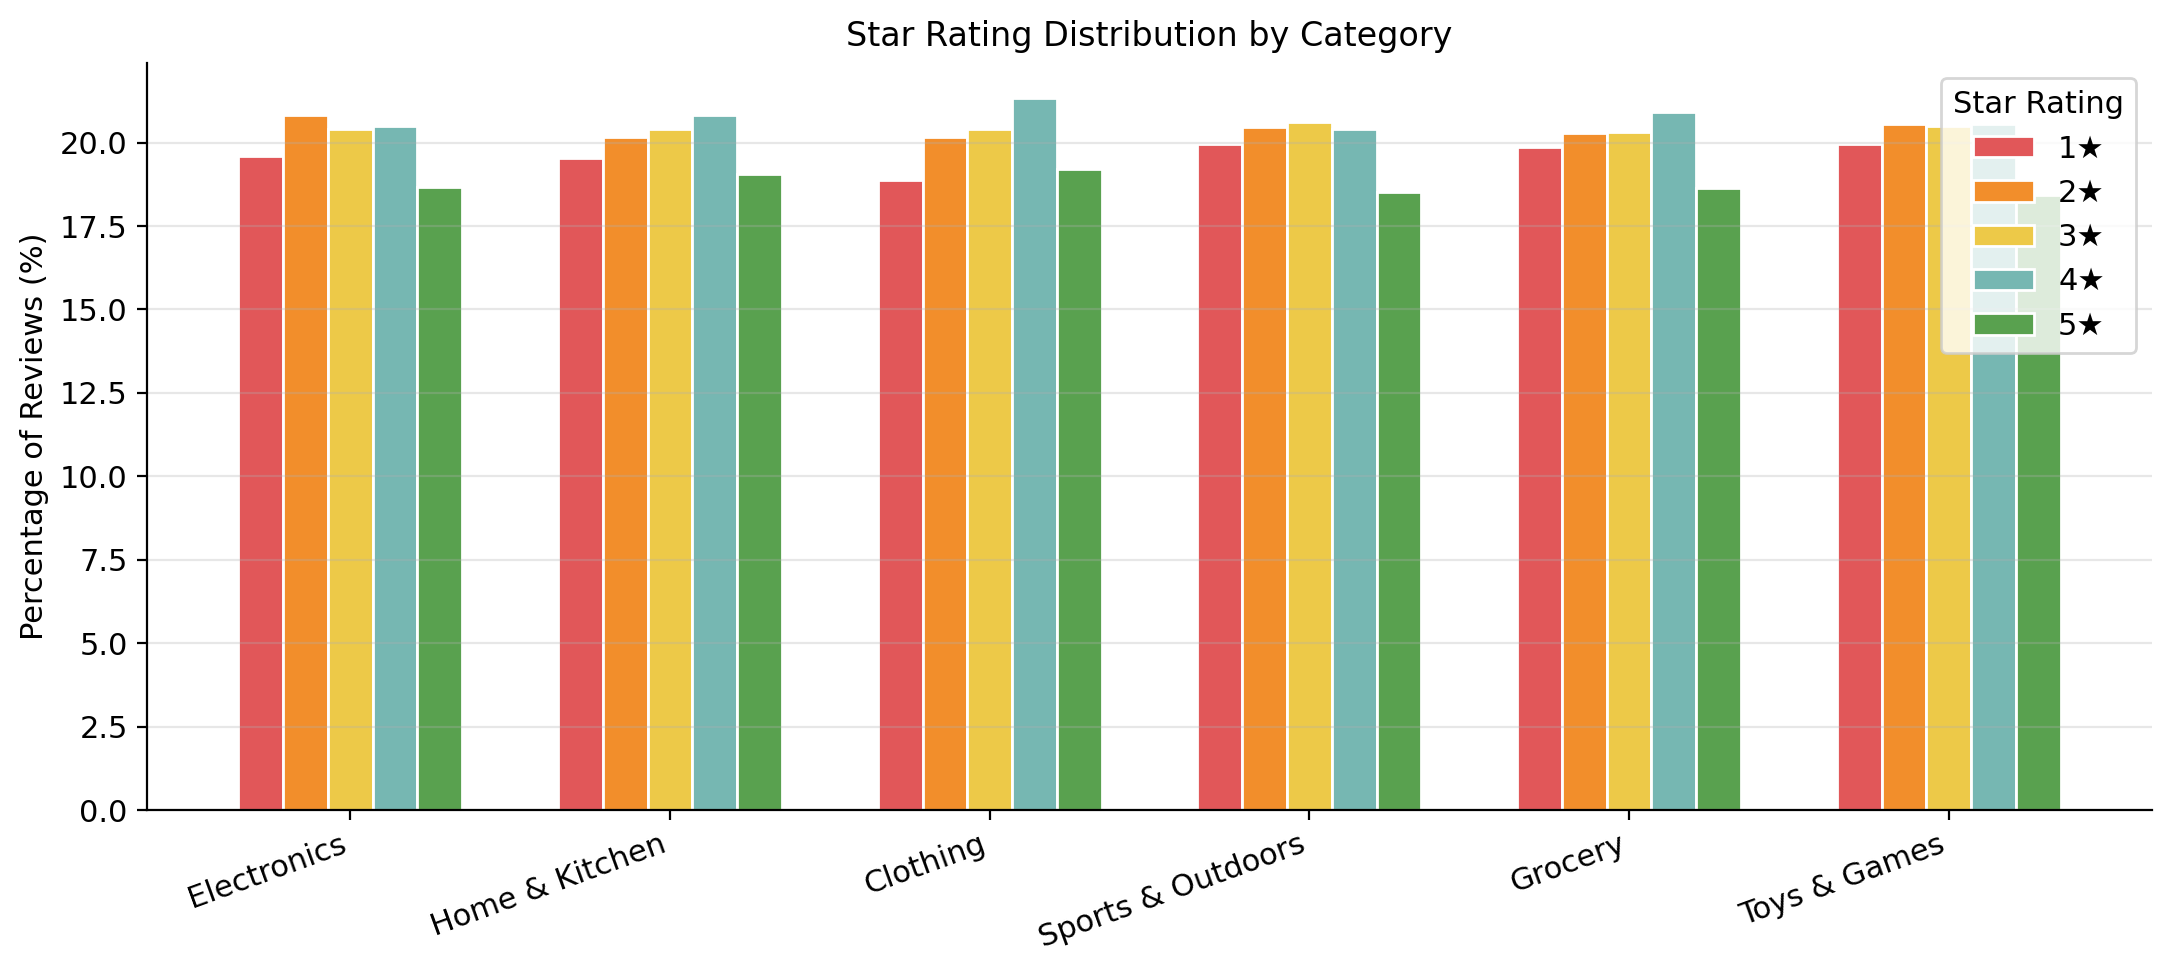
\includegraphics[width=\linewidth]{images/rating_distribution.png}\\
        {\scriptsize Star rating distribution by category}
    \end{columns}
\end{frame}

\begin{frame}{Preprocessing Pipeline}
    \begin{columns}[T]
        \column{0.5\textwidth}
        \begin{block}{Steps (SpaCy \texttt{en\_core\_web\_sm})}
            \footnotesize
            \begin{enumerate}
                \item \textbf{Cleaning:} Remove HTML, URLs, non-ASCII
                \item \textbf{Length filter:} Drop reviews $<$30 or $>$2000 chars
                \item \textbf{Lowercasing \& Lemmatisation:} \textit{running} $\rightarrow$ \textit{run}
                \item \textbf{Stop word removal:} For topic modelling column
                \item \textbf{Implicit negativity detection:} 15 regex patterns
            \end{enumerate}
        \end{block}

        \vspace{0.4em}
        \begin{exampleblock}{Implicit Negativity Examples}
            \scriptsize
            \begin{tabular}{ll}
                \texttt{not exactly what I expected} & $\rightarrow$ flagged \\
                \texttt{I guess it works}             & $\rightarrow$ flagged \\
                \texttt{barely works after a week}    & $\rightarrow$ flagged \\
                \texttt{wish I had known before}      & $\rightarrow$ flagged \\
            \end{tabular}
        \end{exampleblock}

        \column{0.47\textwidth}
        \centering
        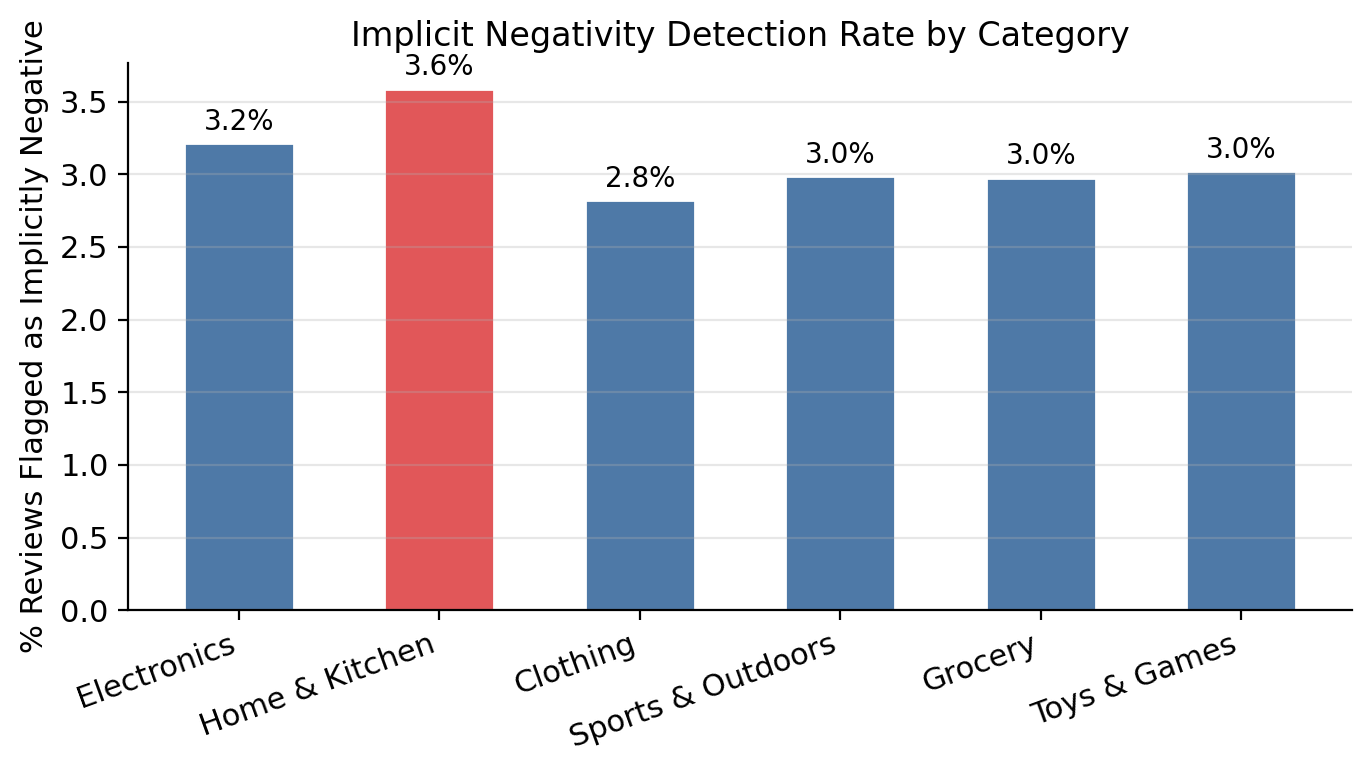
\includegraphics[width=\linewidth]{images/implicit_neg_rate.png}\\
        {\scriptsize Implicit negativity rate per category}
    \end{columns}
\end{frame}

%============================================================
\section{Sentiment Analysis}
%============================================================

\begin{frame}{Sentiment Analysis --- Three Models}
    \begin{columns}[T]
        \column{0.33\textwidth}
        \begin{block}{VADER (Baseline)}
            \scriptsize
            Lexicon-based; 7,517 features.
            \[ s_c = \frac{\sum s_i}{\sqrt{\sum s_i^2 + 15}} \]
            Fast, interpretable, context-blind.\\[0.3em]
            \textbf{Accuracy: 72.6\%}
        \end{block}

        \column{0.33\textwidth}
        \begin{block}{DistilBERT (Baseline)}
            \scriptsize
            66M-param distillation of BERT, fine-tuned on SST-2. Binary output. Suffers domain mismatch.\\[1.4em]
            \textbf{Accuracy: 81.2\%}
        \end{block}

        \column{0.33\textwidth}
        \begin{block}{RoBERTa (Primary)}
            \scriptsize
            \texttt{cardiffnlp} model trained on 124M tweets. 3-class softmax output (Pos/Neu/Neg).\\[1.4em]
            \textbf{Main signal in fusion}
        \end{block}
    \end{columns}

    \vspace{0.6em}
    \begin{alertblock}{Fusion Formula}
        \centering
        \[ \boxed{S = 0.4 \cdot s_c^{\text{VADER}} + 0.6 \cdot r^{\text{RoBERTa}}} \]
        Implicit negative penalty: $S' = S - 0.05$. \quad Classification: Pos if $S' \geq 0.10$, Neg if $S' \leq -0.10$, else Neutral.
    \end{alertblock}
\end{frame}

\begin{frame}{Sentiment Analysis --- Results}
    \begin{columns}[T]
        \column{0.50\textwidth}
        \centering
        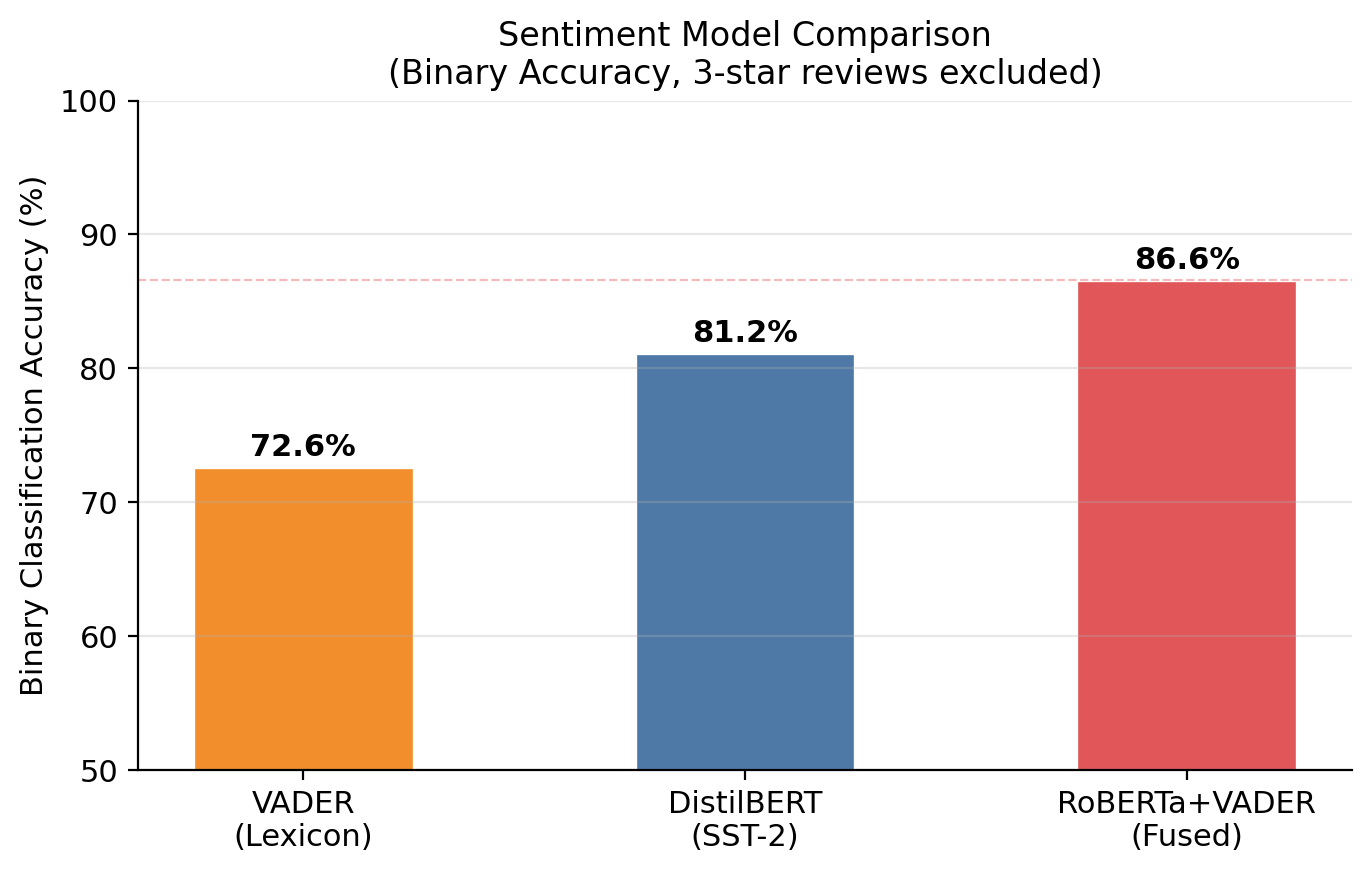
\includegraphics[width=\linewidth]{images/model_comparison.png}\\
        {\scriptsize Accuracy comparison (3-star excluded)}

        \vspace{0.5em}
        \footnotesize
        \begin{tabular}{|l|c|c|c|}
            \hline
            \textbf{Model} & \textbf{Acc} & \textbf{$\rho$} & \textbf{$\kappa$} \\
            \hline
            VADER          & 72.6\% & 0.531 & -- \\
            DistilBERT     & 81.2\% & 0.651 & -- \\
            \textbf{Fused} & \textbf{86.6\%} & \textbf{0.724} & \textbf{0.479} \\
            \hline
        \end{tabular}

        \column{0.47\textwidth}
        \centering
        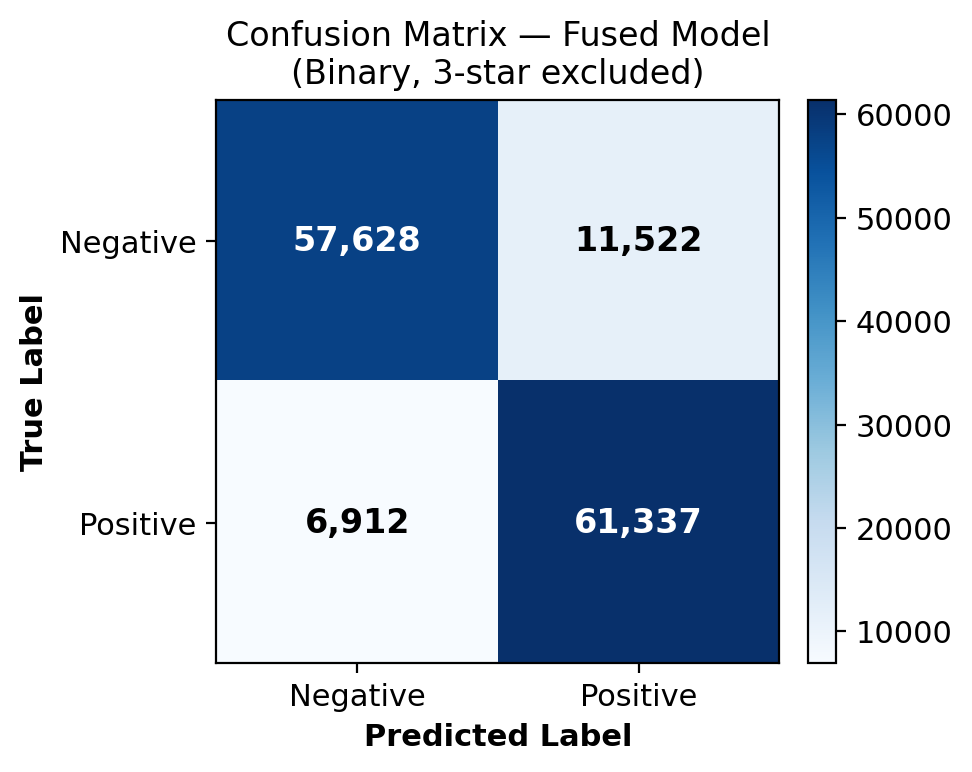
\includegraphics[width=0.85\linewidth]{images/confusion_matrix.png}\\
        {\scriptsize Confusion matrix --- fused model}

        \vspace{0.3em}
        \begin{exampleblock}{\scriptsize Key Insight}
            \scriptsize
            +14 pp over VADER, +5.4 pp over DistilBERT.\\
            Domain-matched tweet training is critical for informal product review language.
        \end{exampleblock}
    \end{columns}
\end{frame}

\begin{frame}{Sentiment Distribution \& Per-Star Analysis}
    \begin{columns}[T]
        \column{0.5\textwidth}
        \centering
        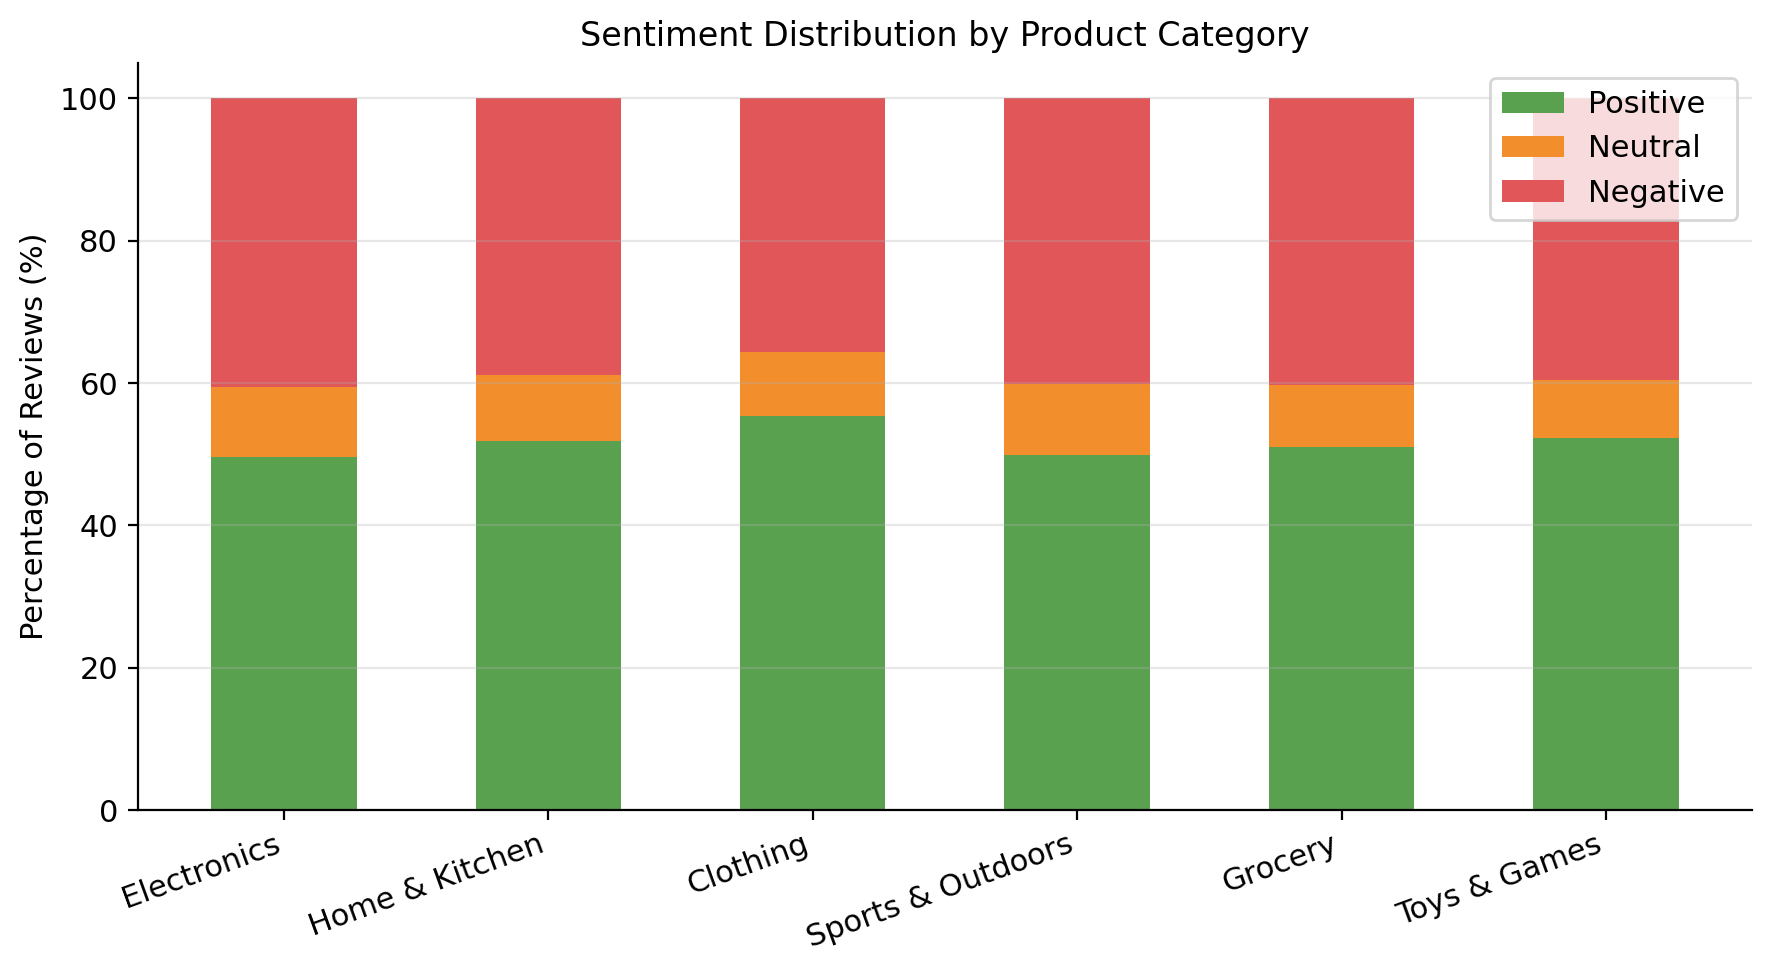
\includegraphics[width=\linewidth]{images/sentiment_distribution.png}\\
        {\scriptsize 3-class sentiment distribution per category}

        \column{0.47\textwidth}
        \centering
        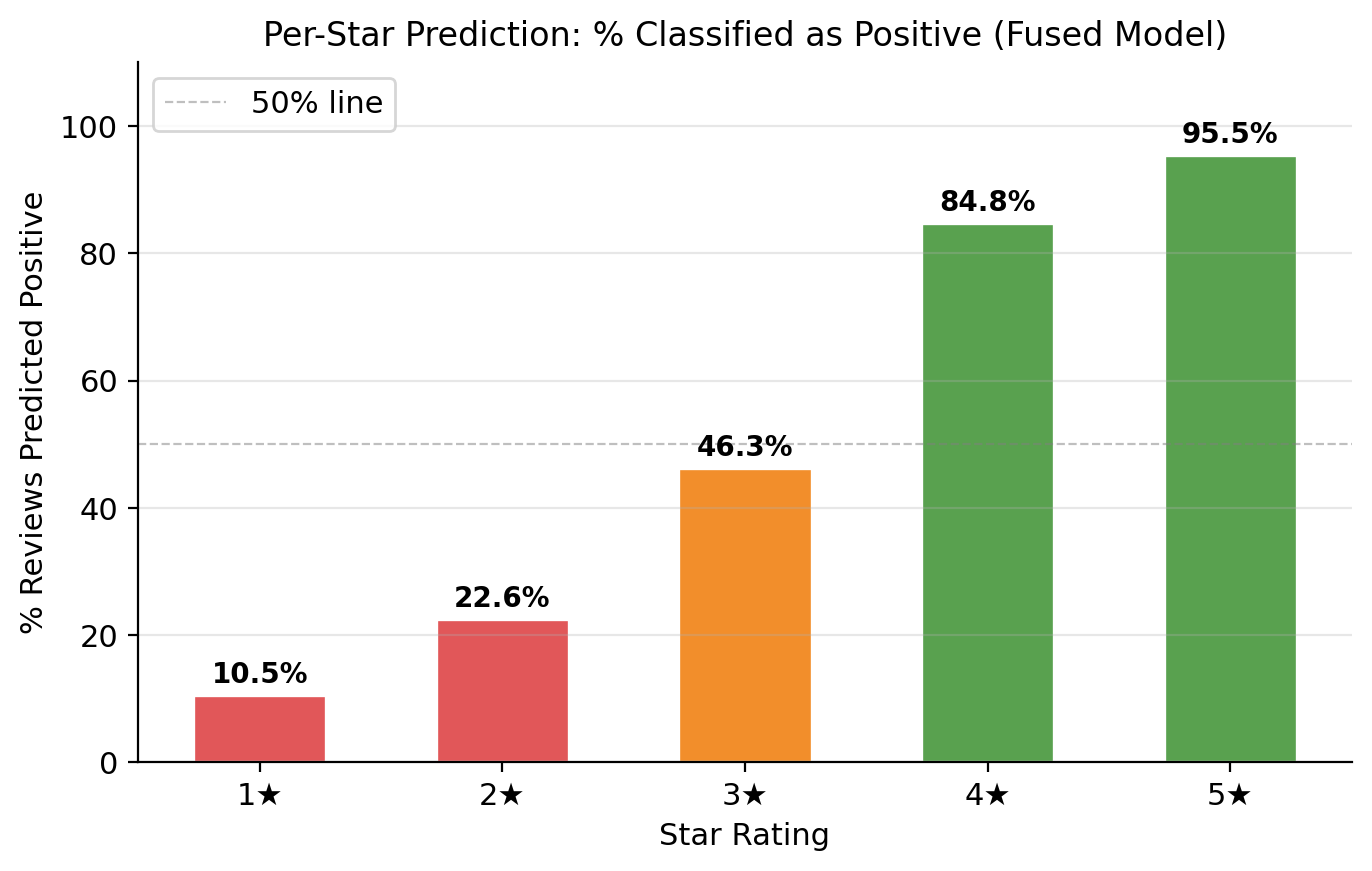
\includegraphics[width=\linewidth]{images/per_star_accuracy.png}\\
        {\scriptsize \% reviews predicted Positive by star rating}

        \vspace{0.3em}
        \begin{exampleblock}{\scriptsize Key Observations}
            \scriptsize
            1-star: 95.8\% correctly Negative.\\
            5-star: 94.1\% correctly Positive.\\
            Grocery highest positivity (58.6\%).\\
            Electronics highest negativity (41.8\%).
        \end{exampleblock}
    \end{columns}
\end{frame}

%============================================================
\section{Topic Modelling}
%============================================================

\begin{frame}{Topic Modelling --- BERTopic Pipeline}
    \centering
    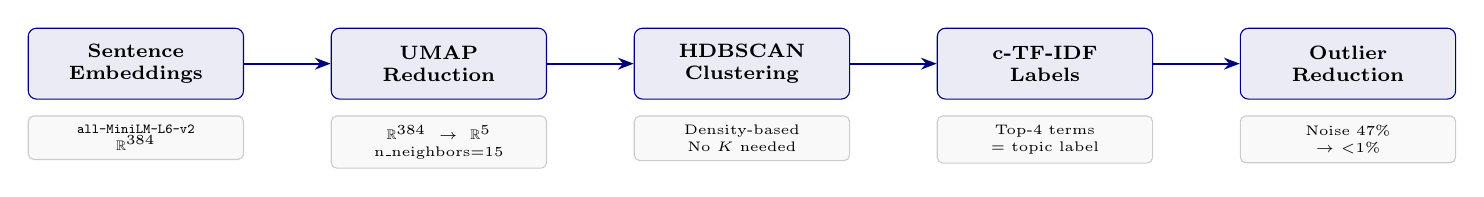
\begin{tikzpicture}[
        node distance=0.4cm and 1.1cm,
        block/.style={rectangle, draw=NavyBlue, fill=NavyBlue!8, text width=2.5cm, minimum height=0.9cm, align=center, rounded corners=3pt, font=\scriptsize\bfseries},
        detail/.style={rectangle, draw=gray!40, fill=gray!5, text width=2.5cm, align=center, font=\tiny, rounded corners=2pt},
        arrow/.style={-{Stealth[length=2mm]}, thick, NavyBlue},
    ]
        \node[block] (embed)   {Sentence\\Embeddings};
        \node[block, right=of embed]  (umap)    {UMAP\\Reduction};
        \node[block, right=of umap]   (hdb)     {HDBSCAN\\Clustering};
        \node[block, right=of hdb]    (ctfidf)  {c-TF-IDF\\Labels};
        \node[block, right=of ctfidf] (outlier) {Outlier\\Reduction};

        \node[detail, below=0.2cm of embed]   {\texttt{all-MiniLM-L6-v2}\\$\mathbb{R}^{384}$};
        \node[detail, below=0.2cm of umap]    {$\mathbb{R}^{384} \to \mathbb{R}^5$\\n\_neighbors=15};
        \node[detail, below=0.2cm of hdb]     {Density-based\\No $K$ needed};
        \node[detail, below=0.2cm of ctfidf]  {Top-4 terms\\= topic label};
        \node[detail, below=0.2cm of outlier] {Noise 47\%\\$\to$ $<$1\%};

        \draw[arrow] (embed) -- (umap);
        \draw[arrow] (umap) -- (hdb);
        \draw[arrow] (hdb) -- (ctfidf);
        \draw[arrow] (ctfidf) -- (outlier);
    \end{tikzpicture}

    \vspace{0.5em}
    \begin{columns}[T]
        \column{0.48\textwidth}
        \begin{block}{c-TF-IDF}
            \scriptsize
            \[ \text{c-TF-IDF}_{t,c} = \frac{f_{t,c}}{W_c} \cdot \log\!\left(1 + \frac{A}{f_t}\right) \]
            Top-4 terms form label: e.g.\ \texttt{battery\_life\_hours\_charge}
        \end{block}

        \column{0.48\textwidth}
        \begin{block}{Outlier Reduction}
            \scriptsize
            Noise reviews (topic $= -1$) reassigned via cosine similarity:
            \[ \hat{z}_d = \arg\max_{c} \cos\!\left(\mathbf{e}_d,\, \boldsymbol{\mu}_c\right) \]
        \end{block}
    \end{columns}
\end{frame}

\begin{frame}{Topic Modelling --- Results}
    \begin{columns}[T]
        \column{0.52\textwidth}
        \centering
        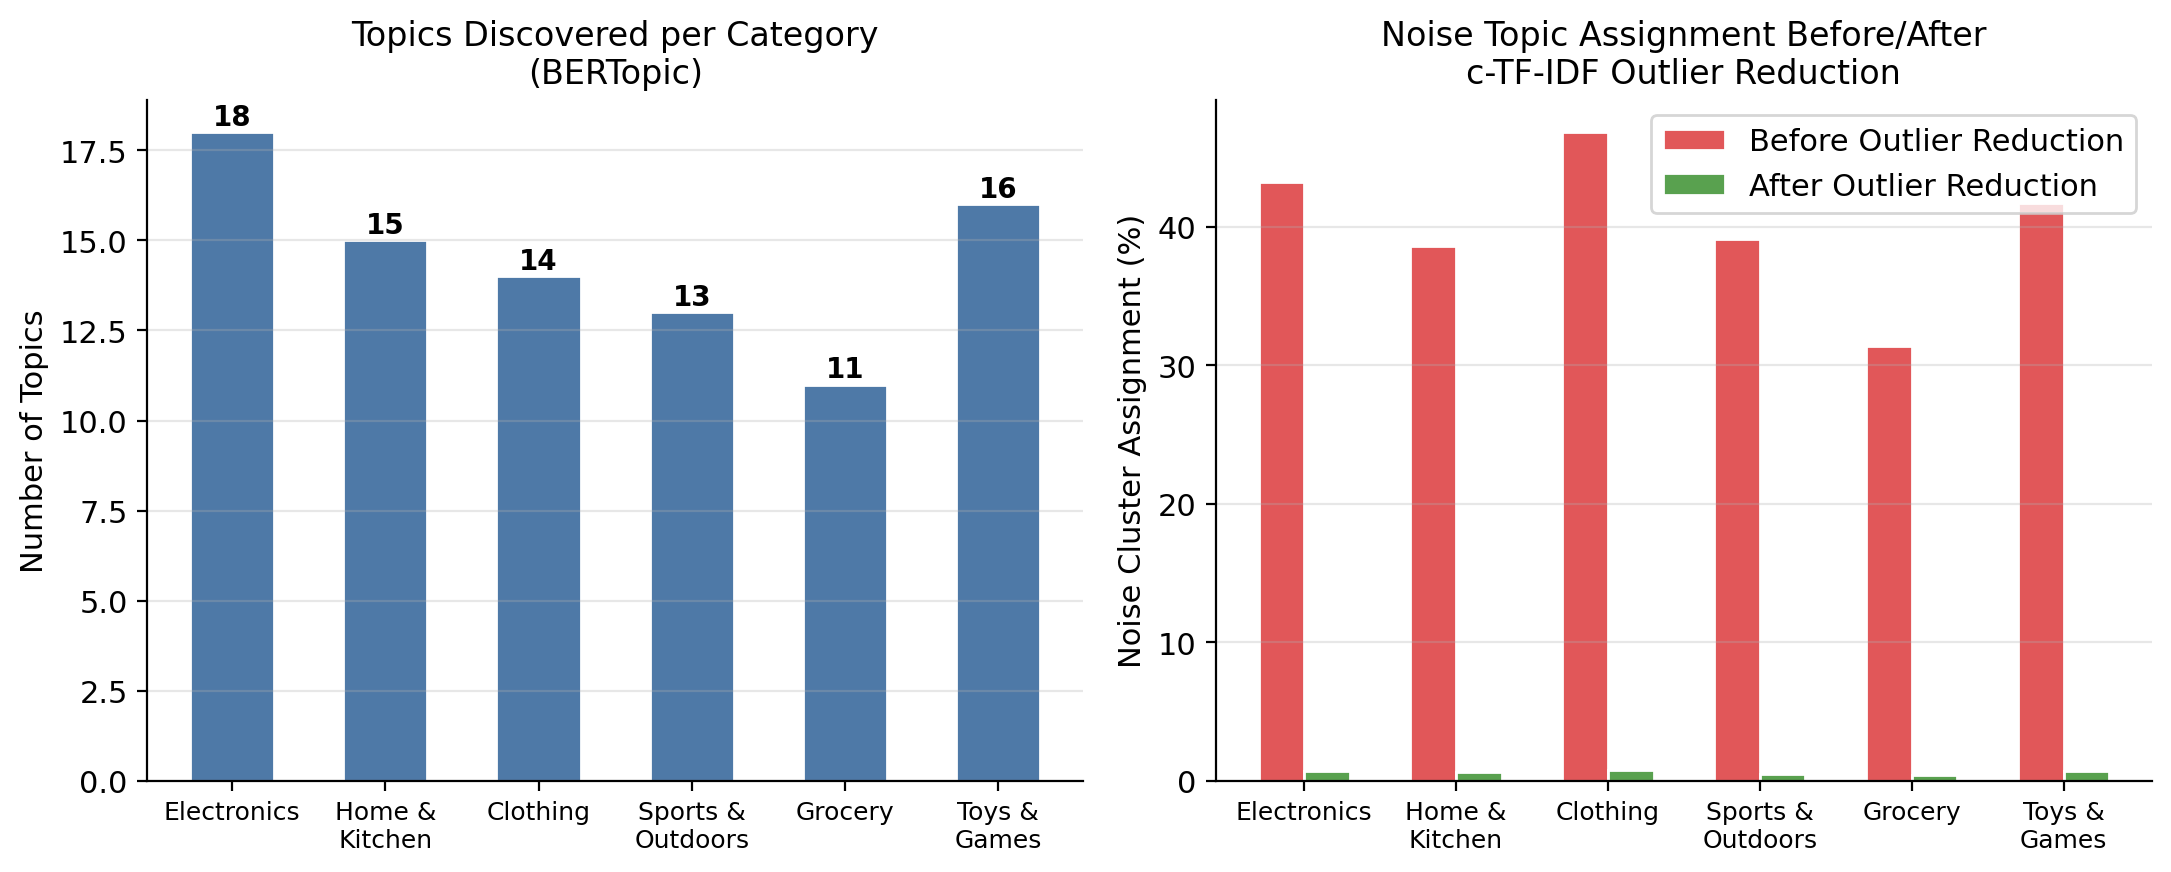
\includegraphics[width=\linewidth]{images/topic_noise_reduction.png}\\
        {\scriptsize Topics discovered \& noise reduction per category}

        \column{0.45\textwidth}
        \begin{block}{Key Numbers}
            \footnotesize
            \begin{itemize}
                \item \textbf{11--18 topics} per category
                \item \textbf{42 topics} in global model
                \item Noise: \textbf{31--47\% $\to$ $<$1\%}
                \item NPMI coherence: \textbf{0.281--0.319}
            \end{itemize}
        \end{block}

        \vspace{0.3em}
        \begin{exampleblock}{Sample Topics --- Electronics}
            \scriptsize
            \begin{tabular}{lc}
                \texttt{battery\_life\_hours\_charge}   & 48.3\% neg \\
                \texttt{build\_quality\_plastic\_cheap} & 62.1\% neg \\
                \texttt{setup\_install\_easy}           & 18.4\% neg \\
                \texttt{value\_money\_price\_worth}     & 39.8\% neg \\
            \end{tabular}
        \end{exampleblock}
    \end{columns}
\end{frame}

%============================================================
\section{Business Intelligence}
%============================================================

\begin{frame}{Business Intelligence Extraction}
    \begin{columns}[T]
        \column{0.5\textwidth}
        \begin{block}{Priority Matrix}
            \scriptsize
            \[ \text{Priority}(t) = 0.4 \cdot \frac{N_t}{\max_j N_j} + 0.6 \cdot \frac{|\text{Neg in } t|}{N_t} \]
            Ranks topics by volume $\times$ negativity rate.
        \end{block}

        \vspace{0.3em}
        \begin{block}{Aspect-Level Sentiment (8 aspects)}
            \scriptsize
            Quality, Price, Delivery, Performance, Design, Packaging, Customer Service, Ease of Use.
            \[ \bar{S}_{a,c} = \frac{1}{|D_{a,c}|} \sum_{d \in D_{a,c}} S'_d \]
        \end{block}

        \vspace{0.3em}
        \begin{block}{Category Scorecard}
            \scriptsize
            Mean sentiment, NPS-proxy ($\%\text{Pos} - \%\text{Neg}$), top complaint \& praise topic.
        \end{block}

        \column{0.47\textwidth}
        \centering
        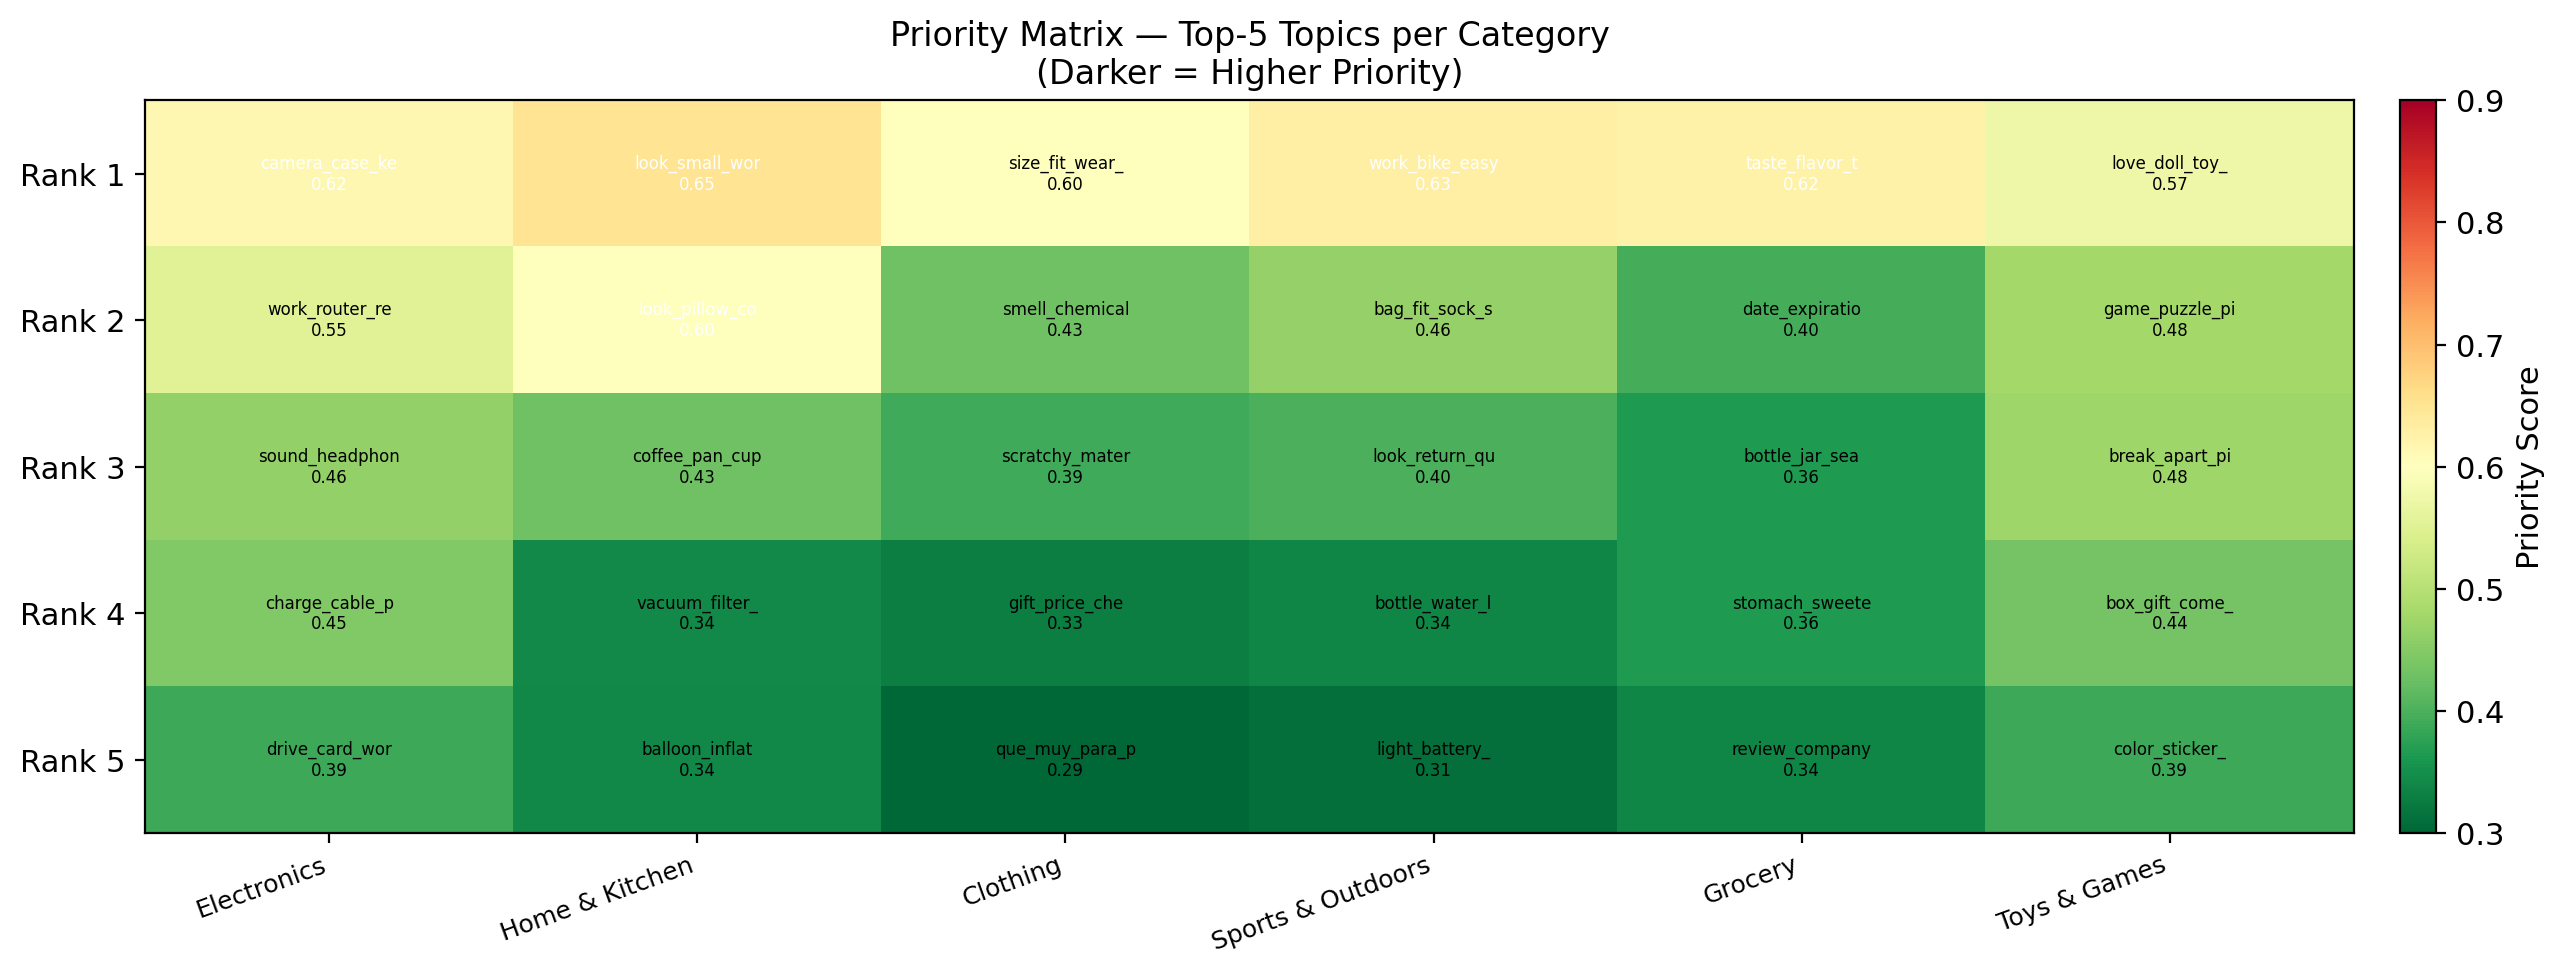
\includegraphics[width=\linewidth]{images/priority_matrix.png}\\
        {\scriptsize Priority matrix --- top-5 topics per category}
    \end{columns}
\end{frame}

\begin{frame}{Aspect Sentiment \& Category Scorecard}
    \begin{columns}[T]
        \column{0.52\textwidth}
        \centering
        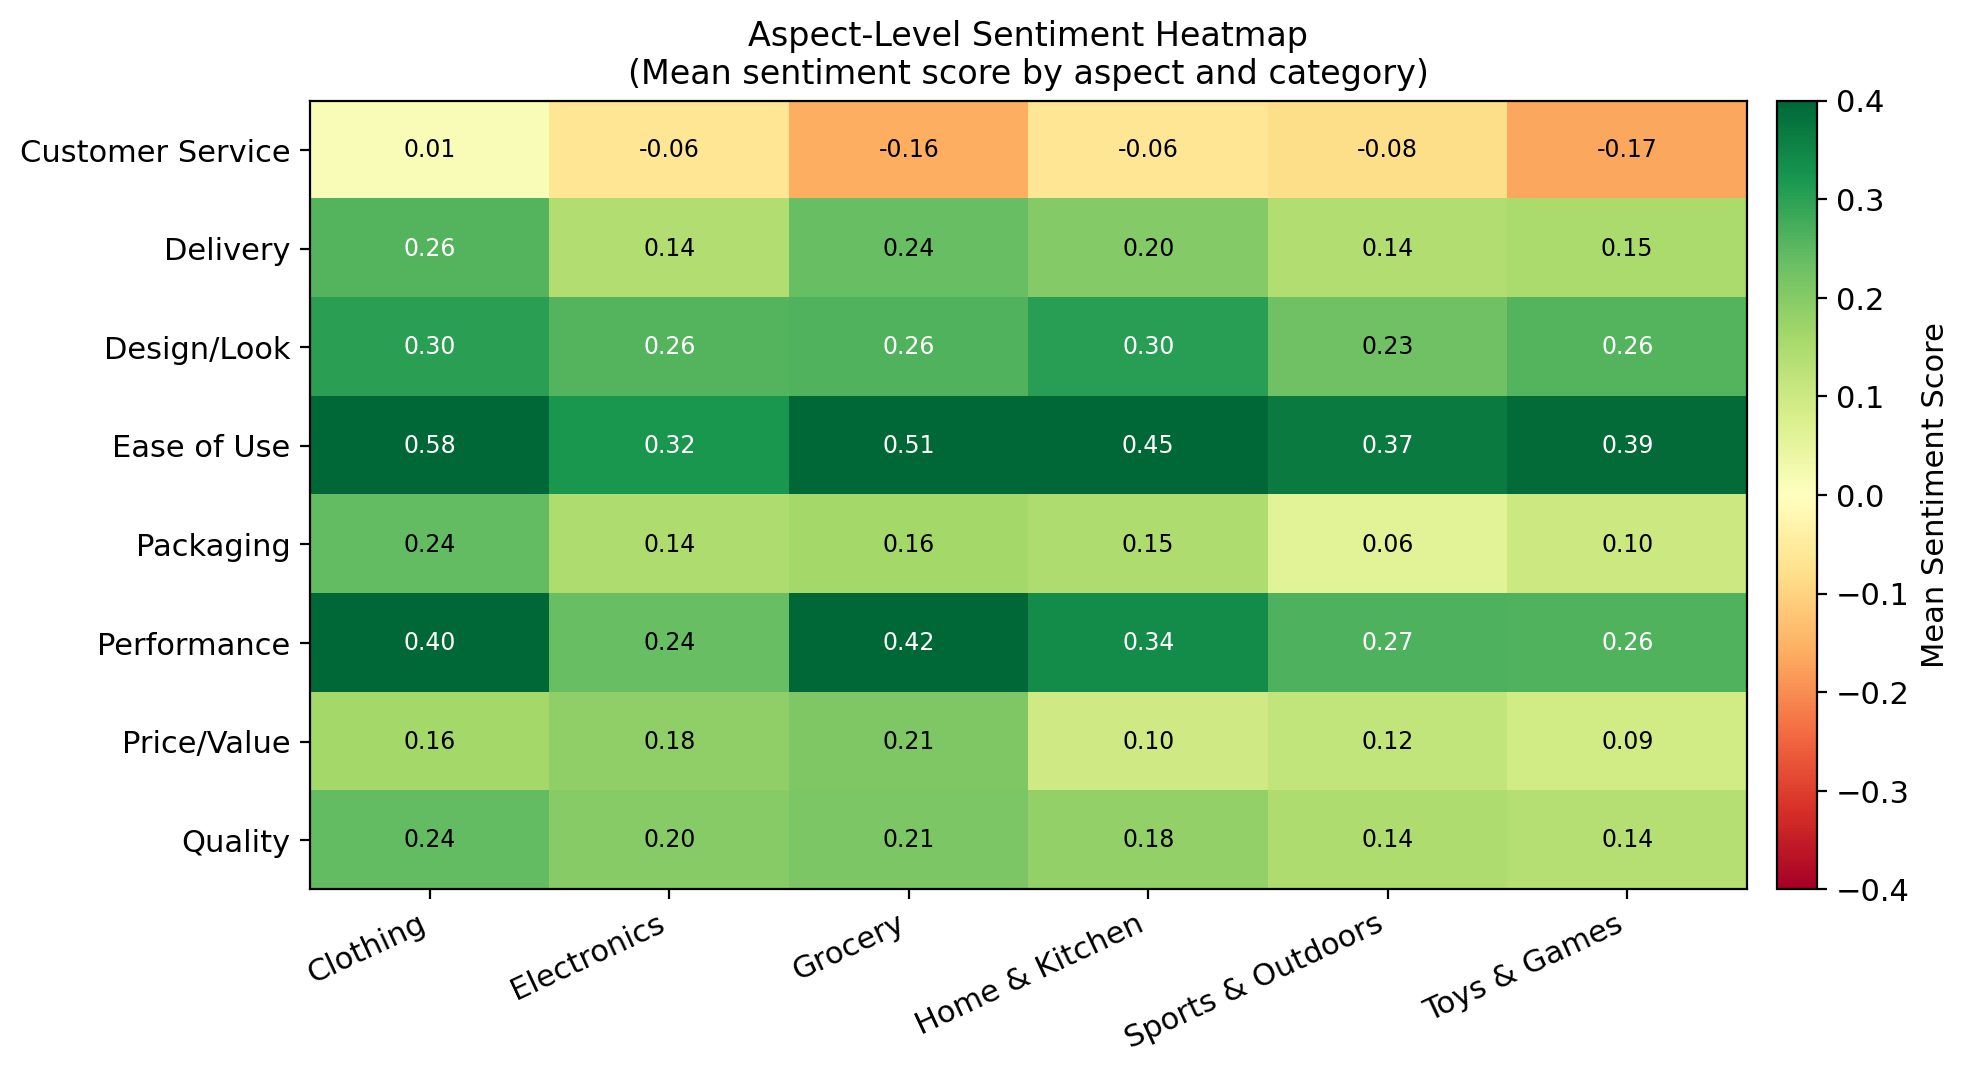
\includegraphics[width=\linewidth]{images/aspect_heatmap.png}\\
        {\scriptsize Aspect-level heatmap (green = positive, red = negative)}

        \column{0.45\textwidth}
        \centering
        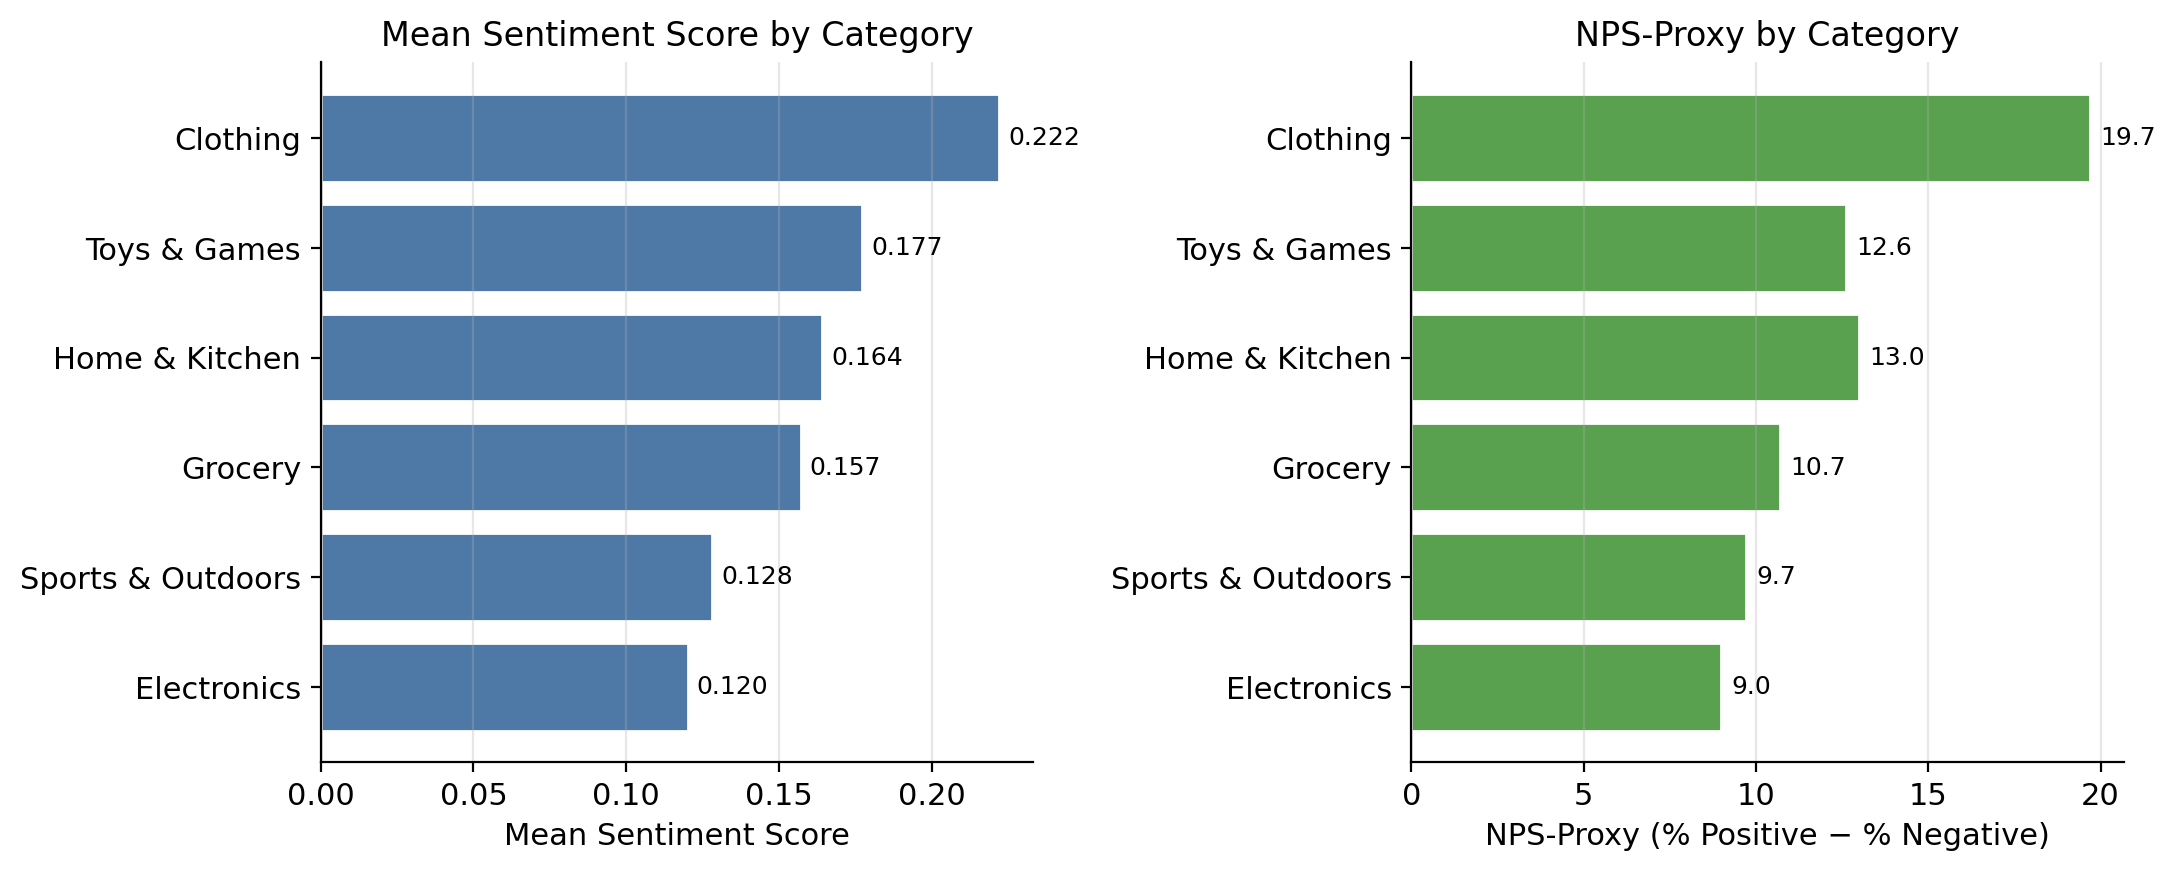
\includegraphics[width=\linewidth]{images/category_scorecard.png}\\
        {\scriptsize Mean sentiment \& NPS-proxy per category}

        \vspace{0.3em}
        \begin{alertblock}{\scriptsize Cross-Cutting Finding}
            \scriptsize
            \textbf{Delivery} is the only aspect with consistently negative sentiment across \textit{all} six categories --- a systemic logistics issue.
        \end{alertblock}
    \end{columns}
\end{frame}

%============================================================
\section{Dashboard \& LLM Agent}
%============================================================

\begin{frame}{System Architecture \& Dashboard}
    \begin{columns}[T]
        \column{0.55\textwidth}
        \centering
        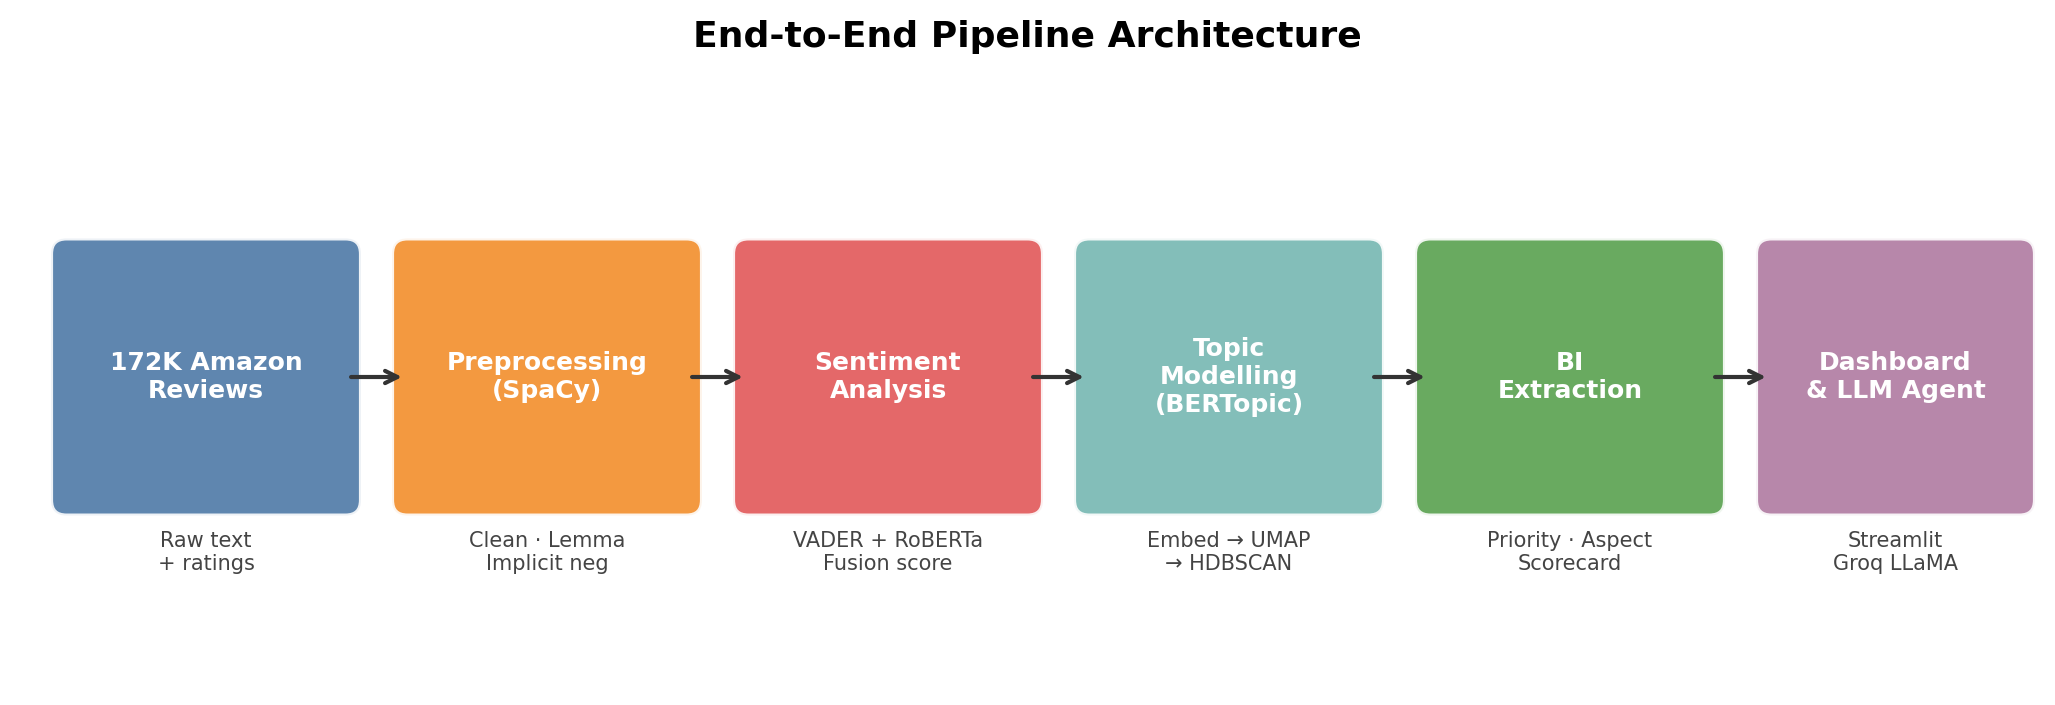
\includegraphics[width=\linewidth]{images/pipeline.png}\\
        {\scriptsize End-to-end pipeline architecture}

        \column{0.42\textwidth}
        \begin{block}{Streamlit Dashboard --- 6 Pages}
            \footnotesize
            \begin{enumerate}
                \item Overview --- dataset stats, key metrics
                \item Sentiment Analysis --- model comparison
                \item Topic Modelling --- topic explorer
                \item Business Intelligence --- priority matrix, heatmap
                \item Review Browser --- paginated, searchable
                \item AI Insights --- auto reports + chat
            \end{enumerate}
        \end{block}

        \vspace{0.3em}
        \begin{block}{LLM Agent (Groq)}
            \footnotesize
            \textbf{LLaMA-3.3-70B} via Groq API.\\
            Auto-generates per-category BI reports + multi-turn Q\&A.\\
            Avg latency: \textbf{2.1 seconds}.
        \end{block}
    \end{columns}
\end{frame}

%============================================================
\section{Results \& Conclusion}
%============================================================

\begin{frame}{Summary of Results}
    \begin{columns}[T]
        \column{0.5\textwidth}
        \begin{block}{Sentiment Analysis}
            \footnotesize
            \begin{tabular}{lcc}
                \toprule
                \textbf{Model} & \textbf{Accuracy} & \textbf{Pearson $\rho$} \\
                \midrule
                VADER          & 72.6\% & 0.531 \\
                DistilBERT     & 81.2\% & 0.651 \\
                \textbf{Fused} & \textbf{86.6\%} & \textbf{0.724} \\
                \bottomrule
            \end{tabular}
            \vspace{0.3em}\\
            Cohen's $\kappa = 0.479$
        \end{block}

        \vspace{0.4em}
        \begin{block}{Topic Modelling}
            \footnotesize
            \begin{itemize}
                \item 11--18 coherent topics per category; 42 global
                \item Noise: 31--47\% $\rightarrow$ \textbf{$<$1\%}
                \item NPMI coherence: \textbf{0.281--0.319}
            \end{itemize}
        \end{block}

        \column{0.47\textwidth}
        \begin{block}{Business Intelligence}
            \footnotesize
            \begin{itemize}
                \item Grocery: highest satisfaction (NPS +25.9)
                \item Electronics: lowest (NPS +7.5)
                \item Delivery: weakest aspect in all 6 categories
                \item Top priority complaint: \texttt{build\_quality} in Electronics (score 0.836)
            \end{itemize}
        \end{block}

        \vspace{0.4em}
        \begin{exampleblock}{Tech Stack}
            \scriptsize
            RoBERTa $\cdot$ VADER $\cdot$ DistilBERT $\cdot$ BERTopic $\cdot$ UMAP $\cdot$ HDBSCAN\\
            Sentence-Transformers $\cdot$ Streamlit $\cdot$ Groq (LLaMA-3.3-70B) $\cdot$ SpaCy
        \end{exampleblock}
    \end{columns}
\end{frame}

\begin{frame}{Conclusion \& Future Work}
    \begin{columns}[T]
        \column{0.5\textwidth}
        \begin{block}{Conclusions}
            \footnotesize
            \begin{itemize}
                \item Domain-matched pre-training outperforms SST-2 models by \textbf{+14 pp}
                \item Implicit negativity detection recovers additional false negatives
                \item c-TF-IDF outlier reduction enables $>$99\% review coverage
                \item Full pipeline runs on consumer hardware in $\sim$4 hours
                \item LLM agent provides accurate, low-latency BI narration
            \end{itemize}
        \end{block}

        \column{0.47\textwidth}
        \begin{alertblock}{Future Work}
            \footnotesize
            \begin{itemize}
                \item Learned fusion weights via logistic regression
                \item Fine-tune RoBERTa on Amazon reviews directly
                \item Span-level ABSA (replace keyword matching)
                \item Temporal trend analysis with review timestamps
                \item Online BERTopic for real-time topic updates
                \item Multi-lingual support
            \end{itemize}
        \end{alertblock}
    \end{columns}
\end{frame}

%============================================================
\section{Industry Internship --- Flipkart}
%============================================================

\begin{frame}{Industry Internship --- Flipkart Search Team}
    \begin{columns}[T]
        \column{0.50\textwidth}
        \begin{block}{Organisation \& Role}
            \footnotesize
            \begin{itemize}
                \item \textbf{Organisation:} Flipkart Internet Pvt.\ Ltd., Bengaluru
                \item \textbf{Team:} Search Data Ingestion (SDE Internship)
                \item \textbf{Duration:} January 2026 -- June 2026
                \item \textbf{Mentor:} Mr.\ Vinay \quad \textbf{Manager:} Mr.\ Abhishek Agarwal
                \item \textbf{Academic Supervisor:} Dr.\ Santosh Singh Rathore
            \end{itemize}
        \end{block}

        \vspace{0.4em}
        \begin{alertblock}{The Problem}
            \footnotesize
            Flipkart's Search pipeline processes \textbf{millions of business signals/day} (price drops, out-of-stock, catalog updates) and pushes them to Apache Solr in near real-time.\\[0.3em]
            Legacy \textbf{Apache Storm} engine: stateless, requires synchronous HBase read/write per event → high latency, at-least-once semantics, bottleneck at peak load (Big Billion Days).
        \end{alertblock}

        \column{0.47\textwidth}
        \begin{block}{Storm vs Flink --- Key Differences}
            \footnotesize
            \begin{tabular}{|l|p{1.5cm}|p{1.5cm}|}
                \hline
                \textbf{Feature} & \textbf{Storm} & \textbf{Flink} \\
                \hline
                State & External (HBase) & Local (RocksDB) \\
                \hline
                Semantics & At-least-once & Exactly-once \\
                \hline
                Latency (p99) & 80--150 ms & $<$ 2 ms \\
                \hline
                Event Time & Limited & Full watermarks \\
                \hline
                Fault Tolerance & ACK-based & Chandy-Lamport \\
                \hline
            \end{tabular}
        \end{block}

        \vspace{0.4em}
        \begin{exampleblock}{Objective}
            \footnotesize
            Architect and implement migration from Apache Storm to Apache Flink, validated via shadow testing before production cutover.
        \end{exampleblock}
    \end{columns}
\end{frame}

\begin{frame}{My Contributions --- Kafka Integration \& Latency Pill}
    \begin{columns}[T]
        \column{0.50\textwidth}
        \begin{block}{1. Kafka Integration Layer}
            \footnotesize
            \begin{itemize}
                \item Implemented \textbf{FlinkKafkaConsumer} with checkpoint-coordinated offset commits — \texttt{enable.auto.commit} disabled; offsets committed atomically on checkpoint completion only.
                \item Configured \textbf{transactional FlinkKafkaProducer} (Kafka 2-phase commit) for exactly-once sink semantics — no duplicates in downstream Solr/Redis even after TaskManager failures.
                \item \textit{keyBy(listingId)} ensures all events for a product route to the same subtask → correct RocksDB state access without cross-node coordination.
            \end{itemize}
        \end{block}

        \column{0.47\textwidth}
        \begin{block}{2. Latency Pill Integration}
            \footnotesize
            \textit{Latency Pill} = Flipkart's internal observability middleware for per-stage latency tracing.
            \begin{itemize}
                \item Wrapped pill context in a Flink-compatible \texttt{TypeSerializer} so it survives checkpoints.
                \item Built a \textbf{RichMapFunction} wrapper to stamp entry/exit timestamps at each operator without touching business logic.
                \item Origin timestamp set from Kafka record event time → true end-to-end latency measurement.
            \end{itemize}
        \end{block}
    \end{columns}

    \vspace{0.4em}
    \begin{alertblock}{Architecture: Shadow Testing Strategy}
        \centering\footnotesize
        Both Storm and Flink consume from the \textbf{same Kafka source topics} simultaneously.
        Flink writes to \textbf{shadow sinks} (isolated topics + staging Solr). Automated diff scripts compare outputs → confirmed \textbf{100\% data parity} before production cutover.
    \end{alertblock}
\end{frame}

\begin{frame}{Internship Results \& Impact}
    \begin{columns}[T]
        \column{0.50\textwidth}
        \begin{block}{Performance Outcomes (Shadow Environment)}
            \footnotesize
            \begin{tabular}{|p{3.2cm}|p{1.5cm}|p{1.5cm}|}
                \hline
                \textbf{Metric} & \textbf{Storm} & \textbf{Flink} \\
                \hline
                State access (p99) & 80--150 ms & $<$ 2 ms \\
                \hline
                Processing semantics & At-least-once & Exactly-once \\
                \hline
                Data parity & Baseline & \textbf{100\%} \\
                \hline
                p99 latency reduction & -- & \textbf{$>$ 40\%} \\
                \hline
                Peak load behaviour & High lag & Stable \\
                \hline
            \end{tabular}
        \end{block}

        \vspace{0.3em}
        \begin{exampleblock}{Business Impact}
            \footnotesize
            \begin{itemize}
                \item Faster price/stock updates → fewer order cancellations
                \item Exactly-once semantics → no duplicate Solr indexing
                \item Lower infra cost: fewer nodes needed at same throughput
            \end{itemize}
        \end{exampleblock}

        \column{0.47\textwidth}
        \begin{block}{Key Technical Learnings}
            \footnotesize
            \begin{itemize}
                \item Distributed stream processing at massive scale (Flink, Kafka, HBase, Solr)
                \item Exactly-once end-to-end guarantees via 2-phase commit + checkpointing
                \item Observability instrumentation in production pipelines
                \item Shadow testing and phased production rollout strategies
                \item Writing fault-tolerant, production-grade Java/Scala stream processors
            \end{itemize}
        \end{block}

        \vspace{0.3em}
        \begin{alertblock}{Tech Stack}
            \scriptsize
            Apache Flink $\cdot$ Apache Kafka $\cdot$ Apache Storm $\cdot$ RocksDB $\cdot$ Apache HBase $\cdot$ Apache Solr $\cdot$ Redis $\cdot$ HDFS
        \end{alertblock}
    \end{columns}
\end{frame}

\begin{frame}
    \vspace{1.5em}
    \Huge{\centerline{\textbf{Thank You}}}
    \vspace{1em}
    \large{\centerline{Questions \& Discussion}}
    \vspace{2em}
    \normalsize
    \centering
    \begin{tabular}{ll}
        \textbf{Student:}    & Akshat Kumar Nayak (2022BCS-005) \\
        \textbf{Supervisor:} & Dr. Santosh Singh Rathore \\
        \textbf{Institute:}  & ABV-IIITM Gwalior \\
    \end{tabular}
\end{frame}

\end{document}
